% NOTE: Chapter 03

\chapter{El Lenguaje}
Esta sección describe el léxico, la sintaxis y la semántica de \texthigh{Lua}. En otras palabras, esta sección describe qué tokens son válidos, cómo pueden combinarse y qué significan sus combinaciones.

Los constructos del lenguaje se explicarán utilizando la notación BNF extendida habitual, en la que \lineCode{\{a\}} significa \texthigh{0} o más \texthigh{a's}, y \lineCode{[a]} significa un \texthigh{a} opcional. Los no terminales se muestran como non-terminal, las palabras clave se muestran como \textbf{kword} y otros símbolos terminales se muestran como '='. La sintaxis completa de \texthigh{Lua} se puede encontrar en la sección 9 al final de este manual.


% NOTE: [Primera sección]------------------------------------------------------
\section{Convenciones léxicas}
\texthigh{Lua} es un lenguaje de formato libre. Ignora los espacios y los comentarios entre elementos léxicos (tokens), excepto como delimitadores entre dos tokens. En el código fuente, \texthigh{Lua} reconoce como espacios los caracteres de espacio en blanco ASCII estándar: espacio, avance de formulario, nueva línea, retorno de carro, tabulación horizontal y tabulación vertical.

Los nombres (también llamados identificadores) en \texthigh{Lua} pueden ser cualquier cadena de letras latinas, dígitos arábigos y guiones bajos, que no comience con un dígito y no sea una palabra reservada. Los identificadores se utilizan para nombrar variables, campos de tablas y etiquetas.

Las siguientes palabras clave están reservadas y no pueden ser utilizadas como nombres:

\begin{center} % Centrar la tabla en el texto
	\begin{tabular}{llllll} % Definición de las columnas y el formato de la tabla
		% \toprule % Línea horizontal superior
		\keyword{and}   & \keyword{break} & \keyword{do}       & \keyword{else}  & \keyword{elseif} & \keyword{end}    \\ % Contenido de la primera fila
		\keyword{false} & \keyword{for}   & \keyword{function} & \keyword{goto}  & \keyword{if}     & \keyword{in}     \\ % Contenido de la segunda fila
		\keyword{local} & \keyword{nil}   & \keyword{not}      & \keyword{or}    & \keyword{repeat} & \keyword{return} \\ % Contenido de la tercera fila
		\keyword{then}  & \keyword{true}  & \keyword{until}    & \keyword{while}                                       \\ % Contenido de la cuarta fila \bottomrule % Línea horizontal inferior
	\end{tabular}
	\label{tab:keywords} % Etiqueta para referenciar la tabla
\end{center}

\texthigh{Lua} es un lenguaje sensible a mayúsculas y minúsculas: \keyword{and} es una palabra reservada, pero 'And' y 'AND' son dos nombres diferentes y válidos. Como convención, los programas deben evitar crear nombres que comiencen con un guión bajo seguido de una o más letras mayúsculas (como \_VERSION).

Las siguientes cadenas de texto representan otros tokens:
\begin{center}
	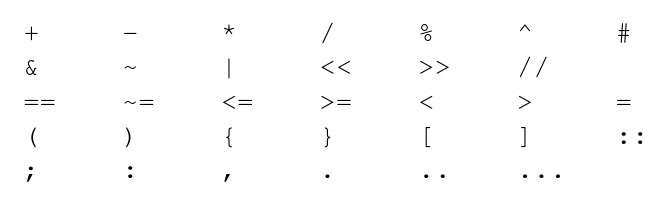
\includegraphics[width=10cm]{chapter3/strings-tokens} % imagen de los tokens
\end{center}

Una cadena de texto corta (literal) puede estar delimitada por comillas simples o comillas dobles y puede contener las siguientes secuencias de escape similares a las de C: '\texthigh{\textbackslash{a}}' (campana), '\texthigh{\textbackslash{b}}' (backspace), '\texthigh{\textbackslash{f}}' (avance de página), '\texthigh{\textbackslash{n}}' (nueva línea), '\texthigh{\textbackslash{r}}' (retorno de carro), '\texthigh{\textbackslash{t}}' (tabulación horizontal), '\texthigh{\textbackslash{v}}' (tabulación vertical), '\texthigh{\textbackslash \textbackslash}' (backslash), '\texthigh{\textbackslash "}' (comilla doble) y '\texthigh{\textbackslash '}' (comilla simple). Si un carácter barra invertida se sigue de un salto de línea, esto resulta en una nueva línea en la cadena de texto. La secuencia de escape '\texthigh{\textbackslash{z}}' omite el siguiente conjunto de caracteres de espacio en blanco, incluyendo saltos de línea; esto es especialmente útil para dividir e indentar una cadena de texto larga en varias líneas sin agregar los saltos de línea y espacios en el contenido de la cadena. Una cadena de texto corta no puede contener saltos de línea no escapados ni secuencias de escape que no formen una secuencia de escape válida.

En una cadena de texto corta (literal), podemos especificar cualquier byte, incluso ceros incrustados, mediante su valor numérico. Esto se puede hacer utilizando la secuencia de escape \texthigh{\textbackslash{xXX}}, donde \texthigh{XX} es una secuencia de exactamente dos dígitos hexadecimales, o con la secuencia de escape \texthigh{\textbackslash{ddd}}, donde \texthigh{ddd} es una secuencia de hasta tres dígitos decimales. (Tenga en cuenta que si una secuencia de escape decimal debe ir seguida de un dígito, debe expresarse con exactamente tres dígitos).

La codificación UTF-8 de un carácter Unicode se puede insertar en una cadena de texto corta (literal) con la secuencia de escape \texthigh{\textbackslash{u\{XXX\}}} (con las llaves obligatorias), donde \texthigh{XXX} es una secuencia de uno o más dígitos hexadecimales que representan el punto de código del carácter. Este punto de código puede tener cualquier valor menor que $2^{31}$. (\texthigh{Lua} utiliza la especificación original de UTF-8 aquí, que no está restringida a puntos de código Unicode válidos).

Las cadenas de texto literales también se pueden definir utilizando un formato largo, que está encerrado por corchetes largos. Definimos un corchete largo de apertura de nivel n como un corchete cuadrado de apertura seguido de n signos de igual seguidos por otro corchete cuadrado de apertura. Así, un corchete largo de apertura de nivel 0 se escribe como \texthigh{[[}, un corchete largo de apertura de nivel 1 se escribe como \texthigh{[=[}, y así sucesivamente. Un corchete largo de cierre se define de manera similar; por ejemplo, un corchete largo de cierre de nivel 4 se escribe como \texthigh{]====]}. Una cadena larga comienza con un corchete largo de apertura de cualquier nivel y termina en el primer corchete largo de cierre del mismo nivel. Puede contener cualquier texto excepto un corchete de cierre del mismo nivel. Las cadenas literales en esta forma entre corchetes pueden extenderse por varias líneas, no interpretan secuencias de escape y ignoran corchetes largos de cualquier otro nivel. Cualquier tipo de secuencia de fin de línea (retorno de carro, nueva línea, retorno de carro seguido de nueva línea o nueva línea seguida de retorno de carro) se convierte en una simple nueva línea. Cuando el corchete largo de apertura está inmediatamente seguido de una nueva línea, la nueva línea no se incluye en la cadena.

Como ejemplo, en un sistema que utiliza ASCII (en el cual '\texthigh{a}' está codificado como 97, newline está codificada como 10 y '\texthigh{1}' está codificado como 49), las cinco cadenas literales siguientes denotan la misma cadena:

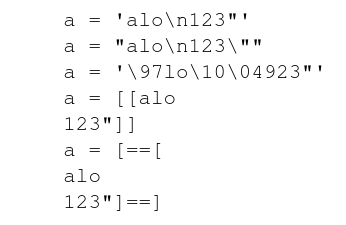
\includegraphics[width=6cm]{chapter3/example01} % imagen de ejemplo

Cualquier byte en una cadena literal que no esté explícitamente afectado por las reglas anteriores se representa tal cual. Sin embargo, \texthigh{Lua} abre archivos para su análisis en modo de texto y las funciones del sistema para archivos pueden tener problemas con algunos caracteres de control. Por lo tanto, es más seguro representar datos binarios como una cadena literal con secuencias de escape explícitas para los caracteres que no son de texto.

Una constante numérica (o numeral) en \texthigh{Lua} puede escribirse con una parte fraccional opcional y un exponente decimal opcional, marcado con una letra '\texthigh{e}' o '\texthigh{E}'. \texthigh{Lua} también acepta constantes hexadecimales, que comienzan con \texthigh{0x} o \texthigh{0X}. Las constantes hexadecimales también pueden tener una parte fraccional opcional y un exponente binario opcional, marcado con una letra '\texthigh{p}' o '\texthigh{P}' y escrito en decimal. (Por ejemplo, \texthigh{0x1}.\texthigh{fp10} representa el número 1984, que es 0x1f dividido con 16 y  multiplicado por $2^{10}$ ---> \lineCode{(0x1f/16)*$2^{10}$}).

Una constante numérica con un punto decimal o un exponente denota un número de tipo "float" (número de punto flotante); de lo contrario, si su valor cabe en un número entero o es una constante hexadecimal, denota un número entero; de lo contrario (es decir, si es un número entero decimal que desborda), denota un número de tipo "float". Los números hexadecimales sin punto decimal ni exponente siempre denotan un valor entero; si el valor desborda, se ajusta para que entre en un entero válido.

Ejemplos de constantes enteras válidas son:

\begin{center}
	\begin{tabular}{llll} % Definición de las columnas y el formato de la tabla
		\texthigh{3} & \texthigh{345} & \texthigh{0xff} & \texthigh{0xBEBADA} \\
	\end{tabular}
	\label{tab:ejemplo} % Etiqueta para referenciar la tabla
\end{center}

Ejemplos de constantes flotantes válidas son:

\begin{center}
	\begin{tabular}{lllll} % Definición de las columnas y el formato de la tabla
		\texthigh{3.0}    & \texthigh{3.1416}   & \texthigh{314.16e-2}            & \texthigh{0.31416E1} & \texthigh{34e1} \\
		\texthigh{0x0.1E} & \texthigh{0xA23p-4} & \texthigh{0X1.921FB54442D18P+1}                                          \\
	\end{tabular}
	\label{tab:ejemplo} % Etiqueta para referenciar la tabla
\end{center}

Un comentario comienza con dos guiones medios ("--) en cualquier lugar fuera de una cadena. Si el texto inmediatamente después de "-- no es un corchete largo de apertura, el comentario es un comentario corto, que se extiende hasta el final de la línea. De lo contrario, es un comentario largo, que se extiende hasta el corchete largo de cierre correspondiente.


% NOTE: [Segunda sección]------------------------------------------------------
\section{Variables}
Las variables son lugares donde se almacenan valores. En \texthigh{Lua}, existen tres tipos de variables: variables globales, variables locales y campos de tablas.

Un solo nombre puede representar una variable global, una variable local (o un parámetro formal de una función, que es un tipo particular de variable local):

\hspace{2cm} \texthigh{var ::= Name}

El nombre denota identificadores (ver \textRef{sección 3.1}).

Cualquier nombre de variable se asume como global a menos que se declare explícitamente como local (ver \textRef{sub-sección 3.3.7}). Las variables locales tienen alcance léxico: las variables locales pueden ser accedidas libremente por las funciones definidas dentro de su alcance (ver \textRef{sección 3.5}).

Antes de la primera asignación a una variable, su valor es \textbf{nil}.

Los corchetes cuadrados se utilizan para indexar una tabla:

\hspace{2cm} \texthigh{var ::= prefixexp} `\textbf{[}` \texthigh{exp} `\textbf{]}`

El significado de los accesos a los campos de una tabla puede ser cambiado mediante las metatablas (ver \textRef{sección 2.4}).

La sintaxis \lineCode{var.Name} es simplemente azúcar sintáctico para \texthigh{var["Nombre"]}:

\hspace{2cm} \texthigh{var ::= prefixexp} `\textbf{.}` \texthigh{Name}

Un acceso a una variable global \texthigh{x} es equivalente a \texthigh{\_ENV.x}. Debido a la forma en que los fragmentos de código son compilados, la variable \texthigh{\_ENV} en sí misma nunca es global (ver \textRef{sección 2.2}).


% NOTE: [Tercera sección]------------------------------------------------------
\section{Sentencias}
\texthigh{Lua} admite un conjunto casi convencional de instrucciones, similar al de otros lenguajes convencionales. Este conjunto incluye bloques de código, asignaciones, estructuras de control, llamadas a funciones y declaraciones de variables.

\subsection{Bloques}
Un bloque es una lista de instrucciones que se ejecutan secuencialmente. En \texthigh{Lua}, un bloque de código está compuesto por una serie de declaraciones o instrucciones que se ejecutan una tras otra en orden. Cada instrucción dentro del bloque se ejecuta en secuencia, una vez que la instrucción anterior ha finalizado.

\hspace{2cm} \texthigh{block ::= \{stat\}}

En Lua, existen las "sentencias vacías" que permiten separar instrucciones con punto y coma, empezar un bloque con un punto y coma o escribir dos puntos y comas en secuencia.

\hspace{2cm} \texthigh{stat ::=} `\textbf{;}`

Por ejemplo, el siguiente código es perfectamente válido en Lua:

\begin{lstlisting}[language=Lua]
    local x = 10;
\end{lstlisting}

Tanto las llamadas a funciones como las asignaciones pueden comenzar con un paréntesis abierto en Lua. Esta posibilidad lleva a una ambigüedad en la gramática de Lua. Considera el siguiente fragmento:

\begin{lstlisting}[language=Lua]
    a = b + c
    (print or io.write)('done')
\end{lstlisting}

La gramática podría interpretar este fragmento de dos formas:

\begin{lstlisting}[language=Lua]
    a = b + c(print or io.write)('done')
    a = b + c; (print or io.write)('done')
\end{lstlisting}

El analizador actual siempre interpreta construcciones de este tipo de la primera manera, considerando el paréntesis abierto como el inicio de los argumentos de una llamada. Para evitar esta ambigüedad, es una buena práctica preceder siempre con un punto y coma a las declaraciones que comienzan con un paréntesis:

\begin{lstlisting}[language=Lua]
    ;(print or io.write)('done')
\end{lstlisting}

Un bloque puede ser delimitado explícitamente para producir una sola declaración:

\begin{lstlisting}[language=Lua]
    stat ::= do block end
\end{lstlisting}

Los bloques explícitos son útiles para controlar el alcance de las declaraciones de variables. También se utilizan a veces bloques explícitos para agregar una declaración de \keyword{return} en medio de otro bloque (ver \textRef{sub-sección 3.3.4}).

\subsection{Fragmentos de Código(Chunks)}
La unidad de compilación de \texthigh{Lua} se llama '\textit{chunk}'. Sintácticamente, un 'chunk' es simplemente un bloque:

\begin{lstlisting}[language=Lua]
    chunk ::= block
\end{lstlisting}

En \texthigh{Lua}, un 'chunk' se maneja como el cuerpo de una función anónima con un número variable de argumentos (ver \textRef{sub-sección 3.4.11}). Como tal, los 'chunks' pueden definir variables locales, recibir argumentos y devolver valores. Además, dicha función anónima se compila en el ámbito de una variable local externa llamada \texthigh{\_ENV} (ver \textRef{sección 2.2}). La función resultante siempre tiene \texthigh{\_ENV} como su única variable externa, incluso si no usa esa variable.

Correcto. En \texthigh{Lua}, un 'chunk' puede ser almacenado en un archivo o en una cadena de texto dentro del programa principal (host program). Para ejecutar un 'chunk', Lua primero lo carga, precompilando el código del 'chunk' en instrucciones para una máquina virtual, y luego ejecuta el código compilado con un intérprete para la máquina virtual.

Los 'chunks' también pueden ser precompilados en forma binaria, lo que se conoce como 'binary chunks'. Para lograr esto, \texthigh{Lua} proporciona un programa llamado \texthigh{luac} que se utiliza para realizar la compilación previa del código fuente en forma binaria. Además, la función \textRef{string.dump} se puede utilizar para precompilar un 'chunk' en una cadena de bytes que representa su forma binaria.

Tanto los programas en forma de código fuente como los compilados en forma binaria son intercambiables en \texthigh{Lua}. Esto significa que puedes cargar y ejecutar tanto 'chunks' en su forma de código fuente (texto) como en su forma precompilada (binaria) utilizando la función \textRef{load}. \texthigh{Lua} automáticamente detectará el tipo de archivo y actuará en consecuencia, lo que proporciona flexibilidad en el manejo de los 'chunks' en diferentes formas.


\subsection{Asignación}
\lipsum[1]

\subsection{Estructuras de Control}
\lipsum[1]

\subsection{Sentencia For}
\lipsum[1]

\subsection{Llamadas de Funciones como Sentencias}
\lipsum[1]

\subsection{Declaraciones Locales}
\lipsum[1]

\subsection{Variables con cierre automático}
\lipsum[1]


% NOTE: [Cuarta sección]------------------------------------------------------
\section{Expresiones}
\lipsum[1-2]

\subsection{Operadores Aritméticos}
\lipsum[1-2]

\subsection{Operadores de Bits}
\lipsum[1-2]

\subsection{Conversiones y Coerciones}
\lipsum[1-2]

\subsection{Operadores Relacionales}
\lipsum[1-2]

\subsection{Operadores Lógicos}
\lipsum[1-2]

\subsection{Concatenación}
\lipsum[1-2]

\subsection{Operador de Longitud}
\lipsum[1-2]

\subsection{Precedencia}
\lipsum[1-2]

\subsection{Constructores de Tablas}
\lipsum[1-2]

\subsection{Llamadas de Funciones}
\lipsum[1-2]

\subsection{Definiciones de Funciones}
\lipsum[1-2]

\subsection{Listas de expresiones, resultados múltiples y ajuste}
\lipsum[1-2]


% NOTE: [Quinta sección]------------------------------------------------------
\section{Reglas de Visibilidad}
\lipsum[1-2]
